\documentclass{article} % A4 paper and 11pt font size
\setcounter{secnumdepth}{0}

\usepackage{amssymb, amsmath, amsfonts}
\usepackage{moreverb}
\usepackage{graphicx}
\usepackage{enumerate}
\usepackage{graphics}
\usepackage[margin=1.25in]{geometry}
\usepackage{color}
\usepackage{tocloft}
\renewcommand{\cftsecleader}{\cftdotfill{\cftdotsep}}
\usepackage{array}
\usepackage{float}
\usepackage{hyperref}
\usepackage{textcomp}
\usepackage[makeroom]{cancel}
\usepackage{bbold}
\usepackage{alltt}
\usepackage{physics}
\usepackage{mathtools}
\usepackage[normalem]{ulem}
\usepackage{amsthm}
\usepackage{tikz}
\usetikzlibrary{positioning}
\usetikzlibrary{arrows}
\usepackage{pgfplots}
\usepackage{bigints}
\allowdisplaybreaks
\pgfplotsset{compat=1.12}

\theoremstyle{plain}
\newtheorem*{theorem*}{Theorem}
\newtheorem{theorem}{Theorem}
\newtheorem*{lemma*}{Lemma}
\newtheorem{lemma}{Lemma}

\makeatletter
\newcommand{\BIGG}{\bBigg@{3}}
\newcommand{\vast}{\bBigg@{4}}
\newcommand{\Vast}{\bBigg@{5}}
\makeatother

\newenvironment{definition}[1][Definition]{\begin{trivlist}
\item[\hskip \labelsep {\bfseries #1}]}{\end{trivlist}}

\newcommand{\E}{\varepsilon}
\def\Rl{\mathbb{R}}
\def\Cx{\mathbb{C}}

\newcommand{\Ei}{\text{Ei}}

\usepackage[T1]{fontenc} % Use 8-bit encoding that has 256 glyphs
\usepackage{fourier} % Use the Adobe Utopia font for the document - comment this line to return to the LaTeX default
\usepackage[english]{babel} % English language/hyphenation

\usepackage{sectsty} % Allows customizing section commands
\allsectionsfont{\centering \normalfont\scshape} % Make all sections centered, the default font and small caps

\usepackage{fancyhdr} % Custom headers and footers
\pagestyle{fancy} % Makes all pages in the document conform to the custom headers and footers
\fancyhead[L]{\bf Sam Fleischer}
\fancyhead[C]{\bf UC Davis \\ Big Data (MAT280)} % No page header - if you want one, create it in the same way as the footers below
\fancyhead[R]{\bf Spring 2016}

\fancyfoot[L]{\bf } % Empty left footer
\fancyfoot[C]{\bf \thepage} % Empty center footer
\fancyfoot[R]{\bf } % Page numbering for right footer
\renewcommand{\headrulewidth}{0pt} % Remove header underlines
\renewcommand{\footrulewidth}{0pt} % Remove footer underlines
\setlength{\headheight}{25pt} % Customize the height of the header

\newcommand{\VEC}[2]{\left\langle #1, #2 \right\rangle}
\newcommand{\ran}{\text{\rm ran }}
\newcommand{\Hilb}{\mathcal{H}}
\newcommand{\lap}{\Delta}

\newcommand{\littleo}[1]{\text{\scriptsize$\mathcal{O}$}\qty(#1)}

\DeclareMathOperator*{\esssup}{\text{ess~sup}}

\newcommand{\problem}[2]{
\vspace{.375cm}
\boxed{\begin{minipage}{\textwidth}
    \section{\bf #1}
    #2
\end{minipage}}
}

\numberwithin{equation}{section} % Number equations within sections (i.e. 1.1, 1.2, 2.1, 2.2 instead of 1, 2, 3, 4)
\numberwithin{figure}{section} % Number figures within sections (i.e. 1.1, 1.2, 2.1, 2.2 instead of 1, 2, 3, 4)
\numberwithin{table}{section} % Number tables within sections (i.e. 1.1, 1.2, 2.1, 2.2 instead of 1, 2, 3, 4)

\setlength\parindent{0pt} % Removes all indentation from paragraphs - comment this line for an assignment with lots of text

\newcommand{\horrule}[1]{\rule{\linewidth}{#1}} % Create horizontal rule command with 1 argument of height

\usepackage{xcolor}
\definecolor{light-gray}{gray}{0.9}

\title{ 
\normalfont \normalsize 
\textsc{UC Davis, Big Data (MAT280), Spring 2016} \\ [25pt] % Your university, school and/or department name(s)
\horrule{2pt} \\[0.4cm] % Thin top horizontal rule
\Huge Homework \#2 \\ % The assignment title
\horrule{2pt} \\[0.5cm] % Thick bottom horizontal rule
}

\author{\huge Sam Fleischer} % Your name

\date{May 2, 2016} % Today's date or a custom date

\begin{document}\thispagestyle{empty}

\maketitle % Print the title

\makeatletter
\@starttoc{toc}
\makeatother

\pagebreak

%%%%%%%%%%%%%%%%%%%%%%%%%%%%%%%%%%%%%%
\problem{Problem 1}{Let $i = \sqrt{-1}$ and set
\begin{align*}
    A = \qty[\begin{array}{ccc}
        i & 0 & -i \\
        0 & i & -i
    \end{array}].
\end{align*}
Using the null space property, show that $\ell_1$-minimization will recover any $1$-sparse vector $x$, given $Ax = y$.}
\begin{proof}
    Given $x = \qty[x_1, x_2, x_3]^T \in \Cx^3$, $Ax = i\qty[x_1 - x_3, x_2 - x_3]^T = 0$ if $x_1 = x_2 = x_3$.  Thus $\text{null} A = \text{span}\qty(\qty[1,1,1]^T)$.  Let $h \in \text{null} A$.  Then $h = \qty[a, a, a]^T$ for some $a \in \Cx$.  Then choose $S_i = \{i\}$ for $i = 1, 2, 3$.  Then
    \begin{align*}
        h_{S_1} = \qty[\begin{array}{c} a\\0\\0\end{array}], \qquad h_{S_2} = \qty[\begin{array}{c} 0\\a\\0\end{array}], \qquad \text{and} \qquad h_{S_3} = \qty[\begin{array}{c} 0\\0\\a \end{array}]
    \end{align*}
    which gives
    \begin{align*}
        h_{S_1^C} = \qty[\begin{array}{c} 0\\a\\a \end{array}], \qquad h_{S_2^C} = \qty[\begin{array}{c} a\\0\\a \end{array}], \qquad \text{and} \qquad h_{S_3^C} = \qty[\begin{array}{c} a\\a\\0 \end{array}]
    \end{align*}
    Clearly $\norm{h_{S_i}}_1 = \abs{a}$ and $\norm{h_{S_i^C}}_1 = 2\abs{a}$ for $i = 1, 2, 3$.  Thus $\norm{h_S}_1 \leq \norm{h_{S^C}}_1$ for all $h \in \text{null} A$ and all $S \subset \{1,2,3\}$ with $\abs{S} = 1$.  This shows the null space property holds and hence $\ell_1$-minimization will recover any $1$-sparse vector $x$.
\end{proof}
    







%%%%%%%%%%%%%%%%%%%%%%%%%%%%%%%%%%%%%%
\problem{Problem 2}{On the connection between (in)coherence parameter $\mu$ and restricted isometry constant $\delta_s$: Show that $\delta_1 = 0$, $\delta_2 = \mu$, and $\delta_s \leq (s-1)\mu$.}
\begin{proof}
\end{proof}
    







%%%%%%%%%%%%%%%%%%%%%%%%%%%%%%%%%%%%%%
\problem{Problem 3}{Let $A = \Rl^{k\times d}$ be a Gaussian random matrix.  Given an estimate for the coherence $\mu$ of $A$.}
\begin{proof}
\end{proof}
    







%%%%%%%%%%%%%%%%%%%%%%%%%%%%%%%%%%%%%%
\problem{Problem 4}{Consider $y = Ax$, where $A$ is a $100 \times 400$ Gaussian random matrix and $x$ is a $s$-sparse vector of length $400$.  The locations of the non-zero entries of $x$ are chosen uniformly at random and the non-zero coefficients of $x$ are normal-distributed.  For $s = 1, 2, \dots, $ solve
\begin{align*}
    \min_z \norm{z}_1 \qquad \text{subject to } Az = y,
\end{align*}
(e.g.~using the toolbox CVX).  For each fixed $s$ repeat the experiment $10$ times.  Create a graph plotting $s$ versus the relative reconstruction error (averaged over the ten experiments for each $s$).  Starting with which value of $s$ approximately does $\ell_1$-minimization fail to recover $x$?}
\begin{proof}
    The following graph shows the mean $\ell^2$-norm errors of $10$ experiments at each $s$ for $s = 1, 2, \dots, 40$.  The non-zero entries of $x$ are normally distributed around $0$ with standard deviation of $1$.
    \begin{figure}[ht!]
        \centering
        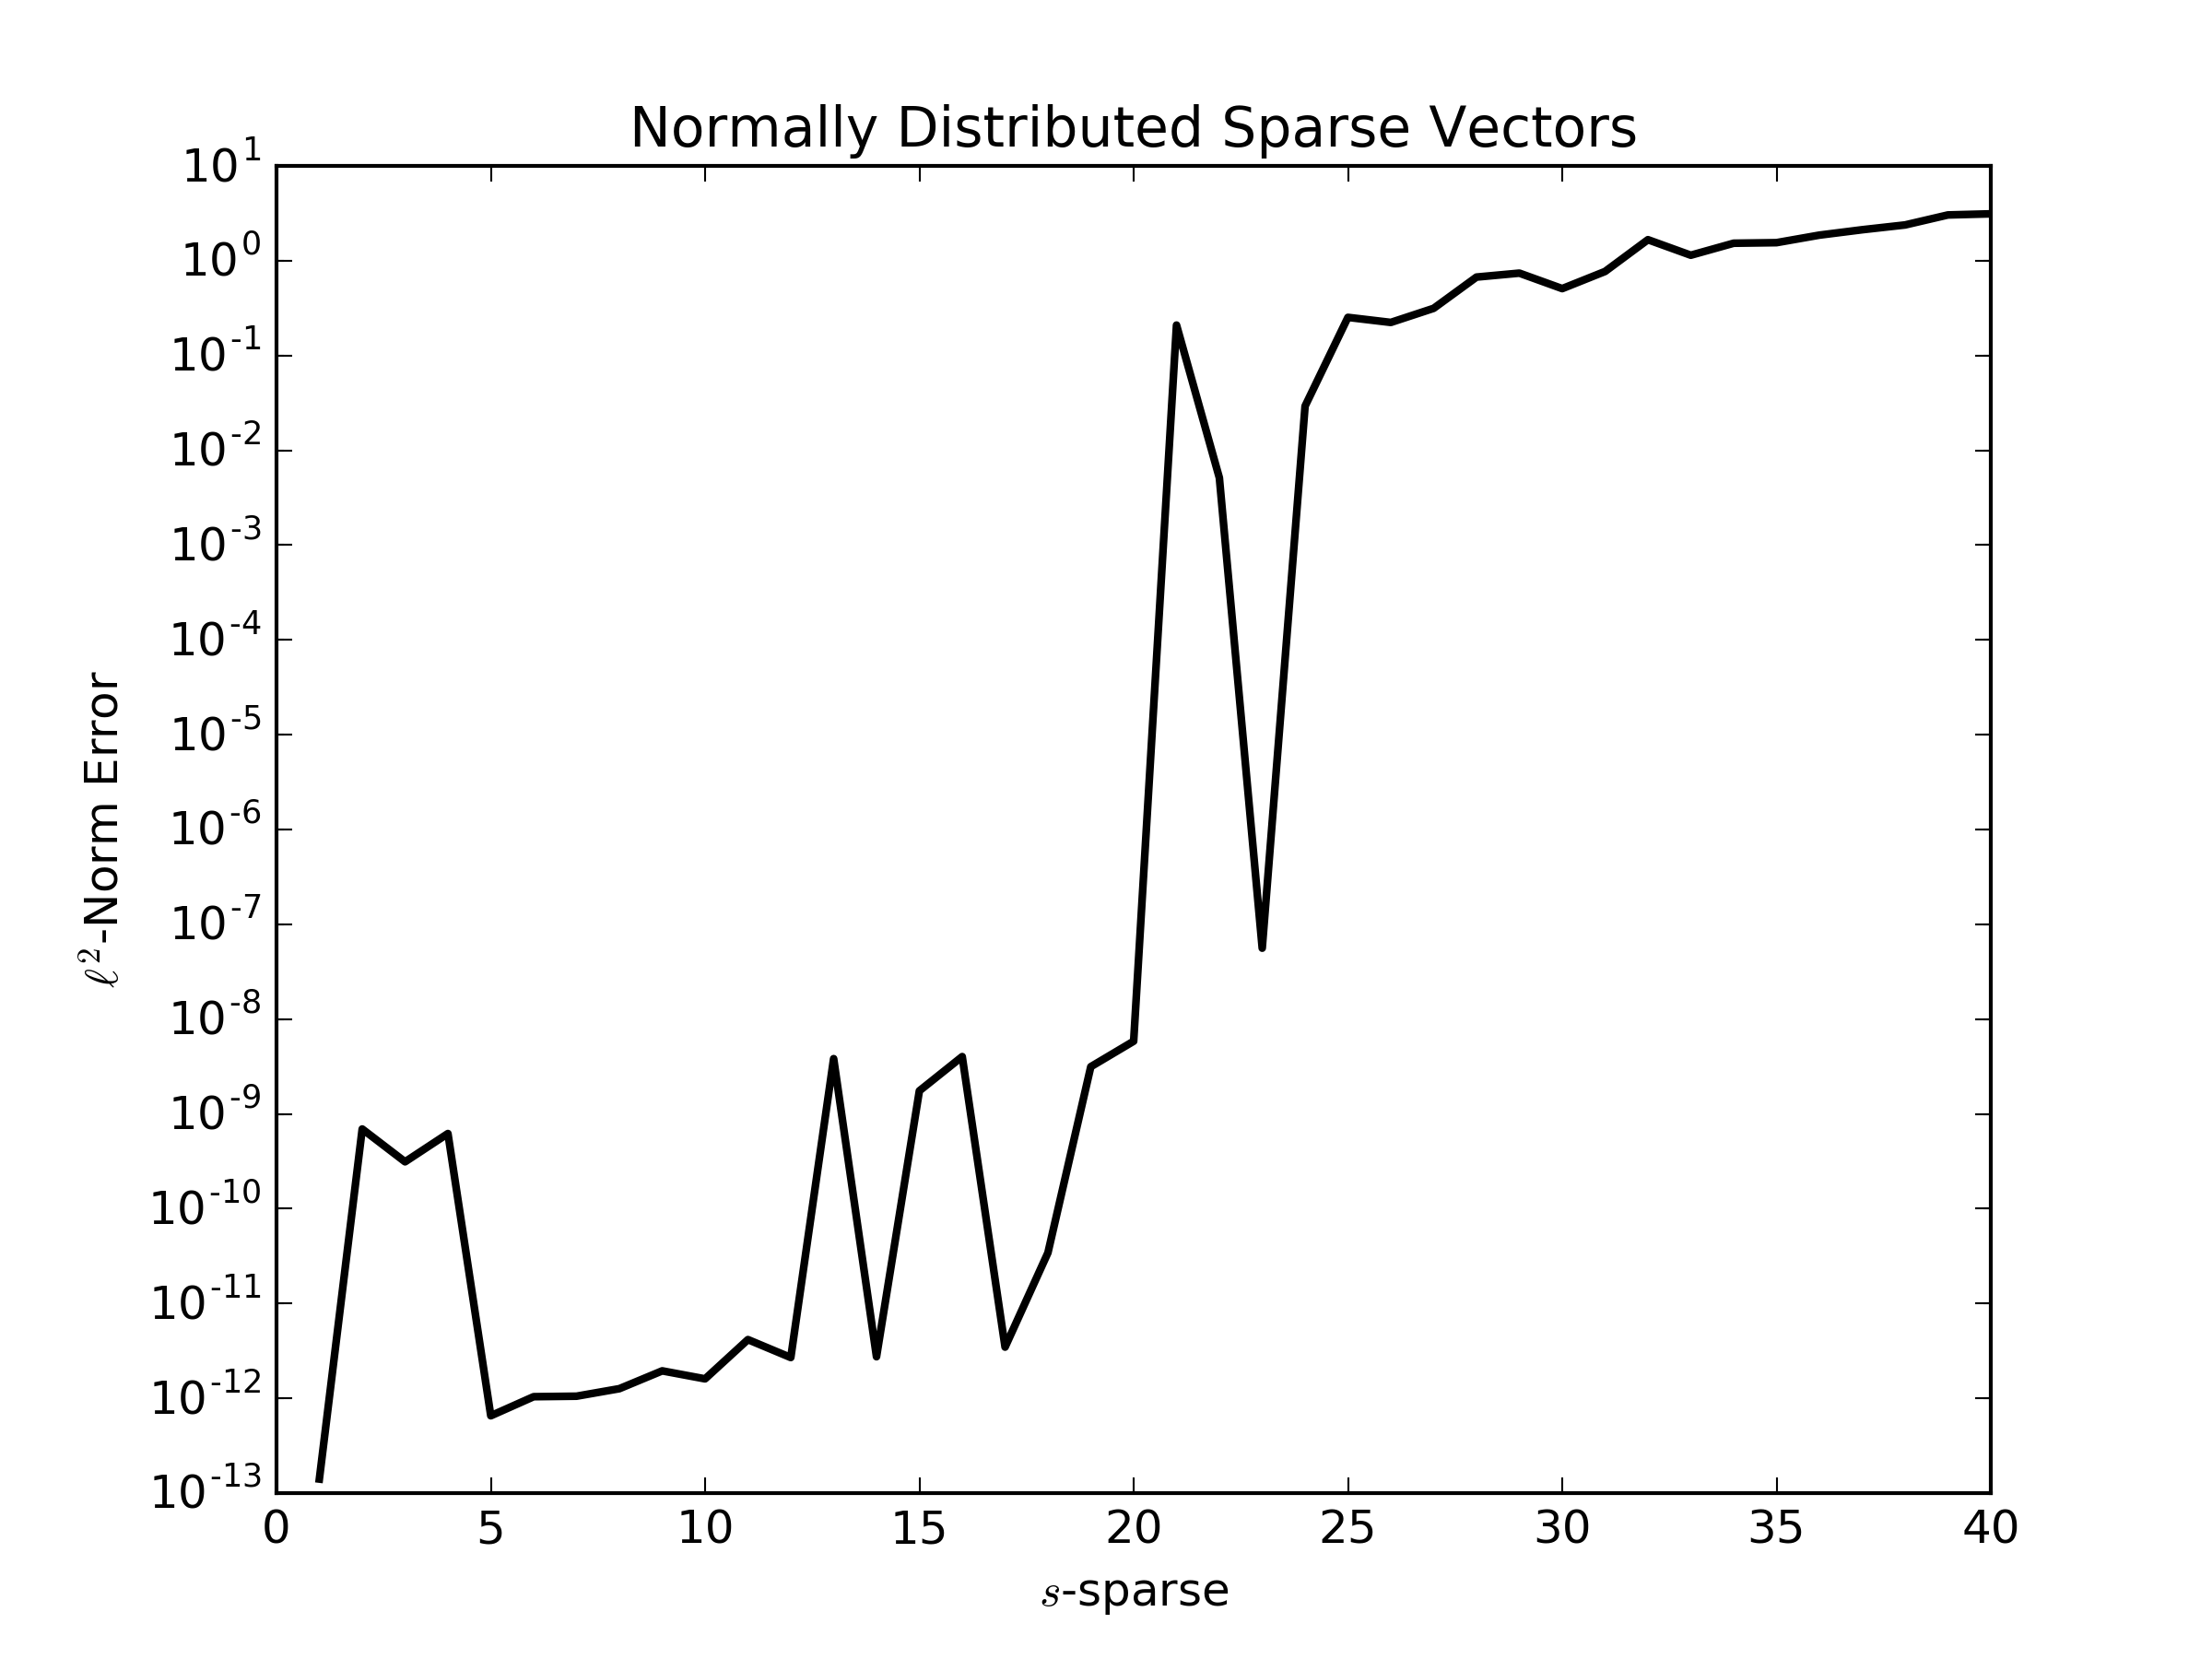
\includegraphics[width=\textwidth]{normally_distributed.png}
    \end{figure}
    In this experiment, this method failed for $s \geq 21$.
\end{proof}
    







%%%%%%%%%%%%%%%%%%%%%%%%%%%%%%%%%%%%%%
\problem{Problem 5}{Same setup as in Problem $4$, but now the non-zero entries of $x$ are non-negative.  Taking this information into account, we now solve
\begin{align*}
    \min_z \norm{z}_1 \qquad \text{subject to } Ax = y \text{ and } z \geq 0
\end{align*}
(here, $z \geq 0$ is meant entrywise, i.e., for each $k$, $z_k \geq 0$).  (The positivity constraint is easy to include in CVX).  Repeat the simulations as described in Problem 4.  Compare your findings to the results from your experiments of Problem 4 and try to quantify the difference regarding the range for $s$ for which recovery is still possible in this case.}
\begin{proof}
    The following graph shows the mean $\ell^2$-norm errors of $10$ experiments at each $s$ for $s = 1, 2, \dots, 40$.  The non-zero entries of $x$ are the absolute value of a normal distribution around $0$ with standard deviation of $1$.
    \begin{figure}[ht!]
        \centering
        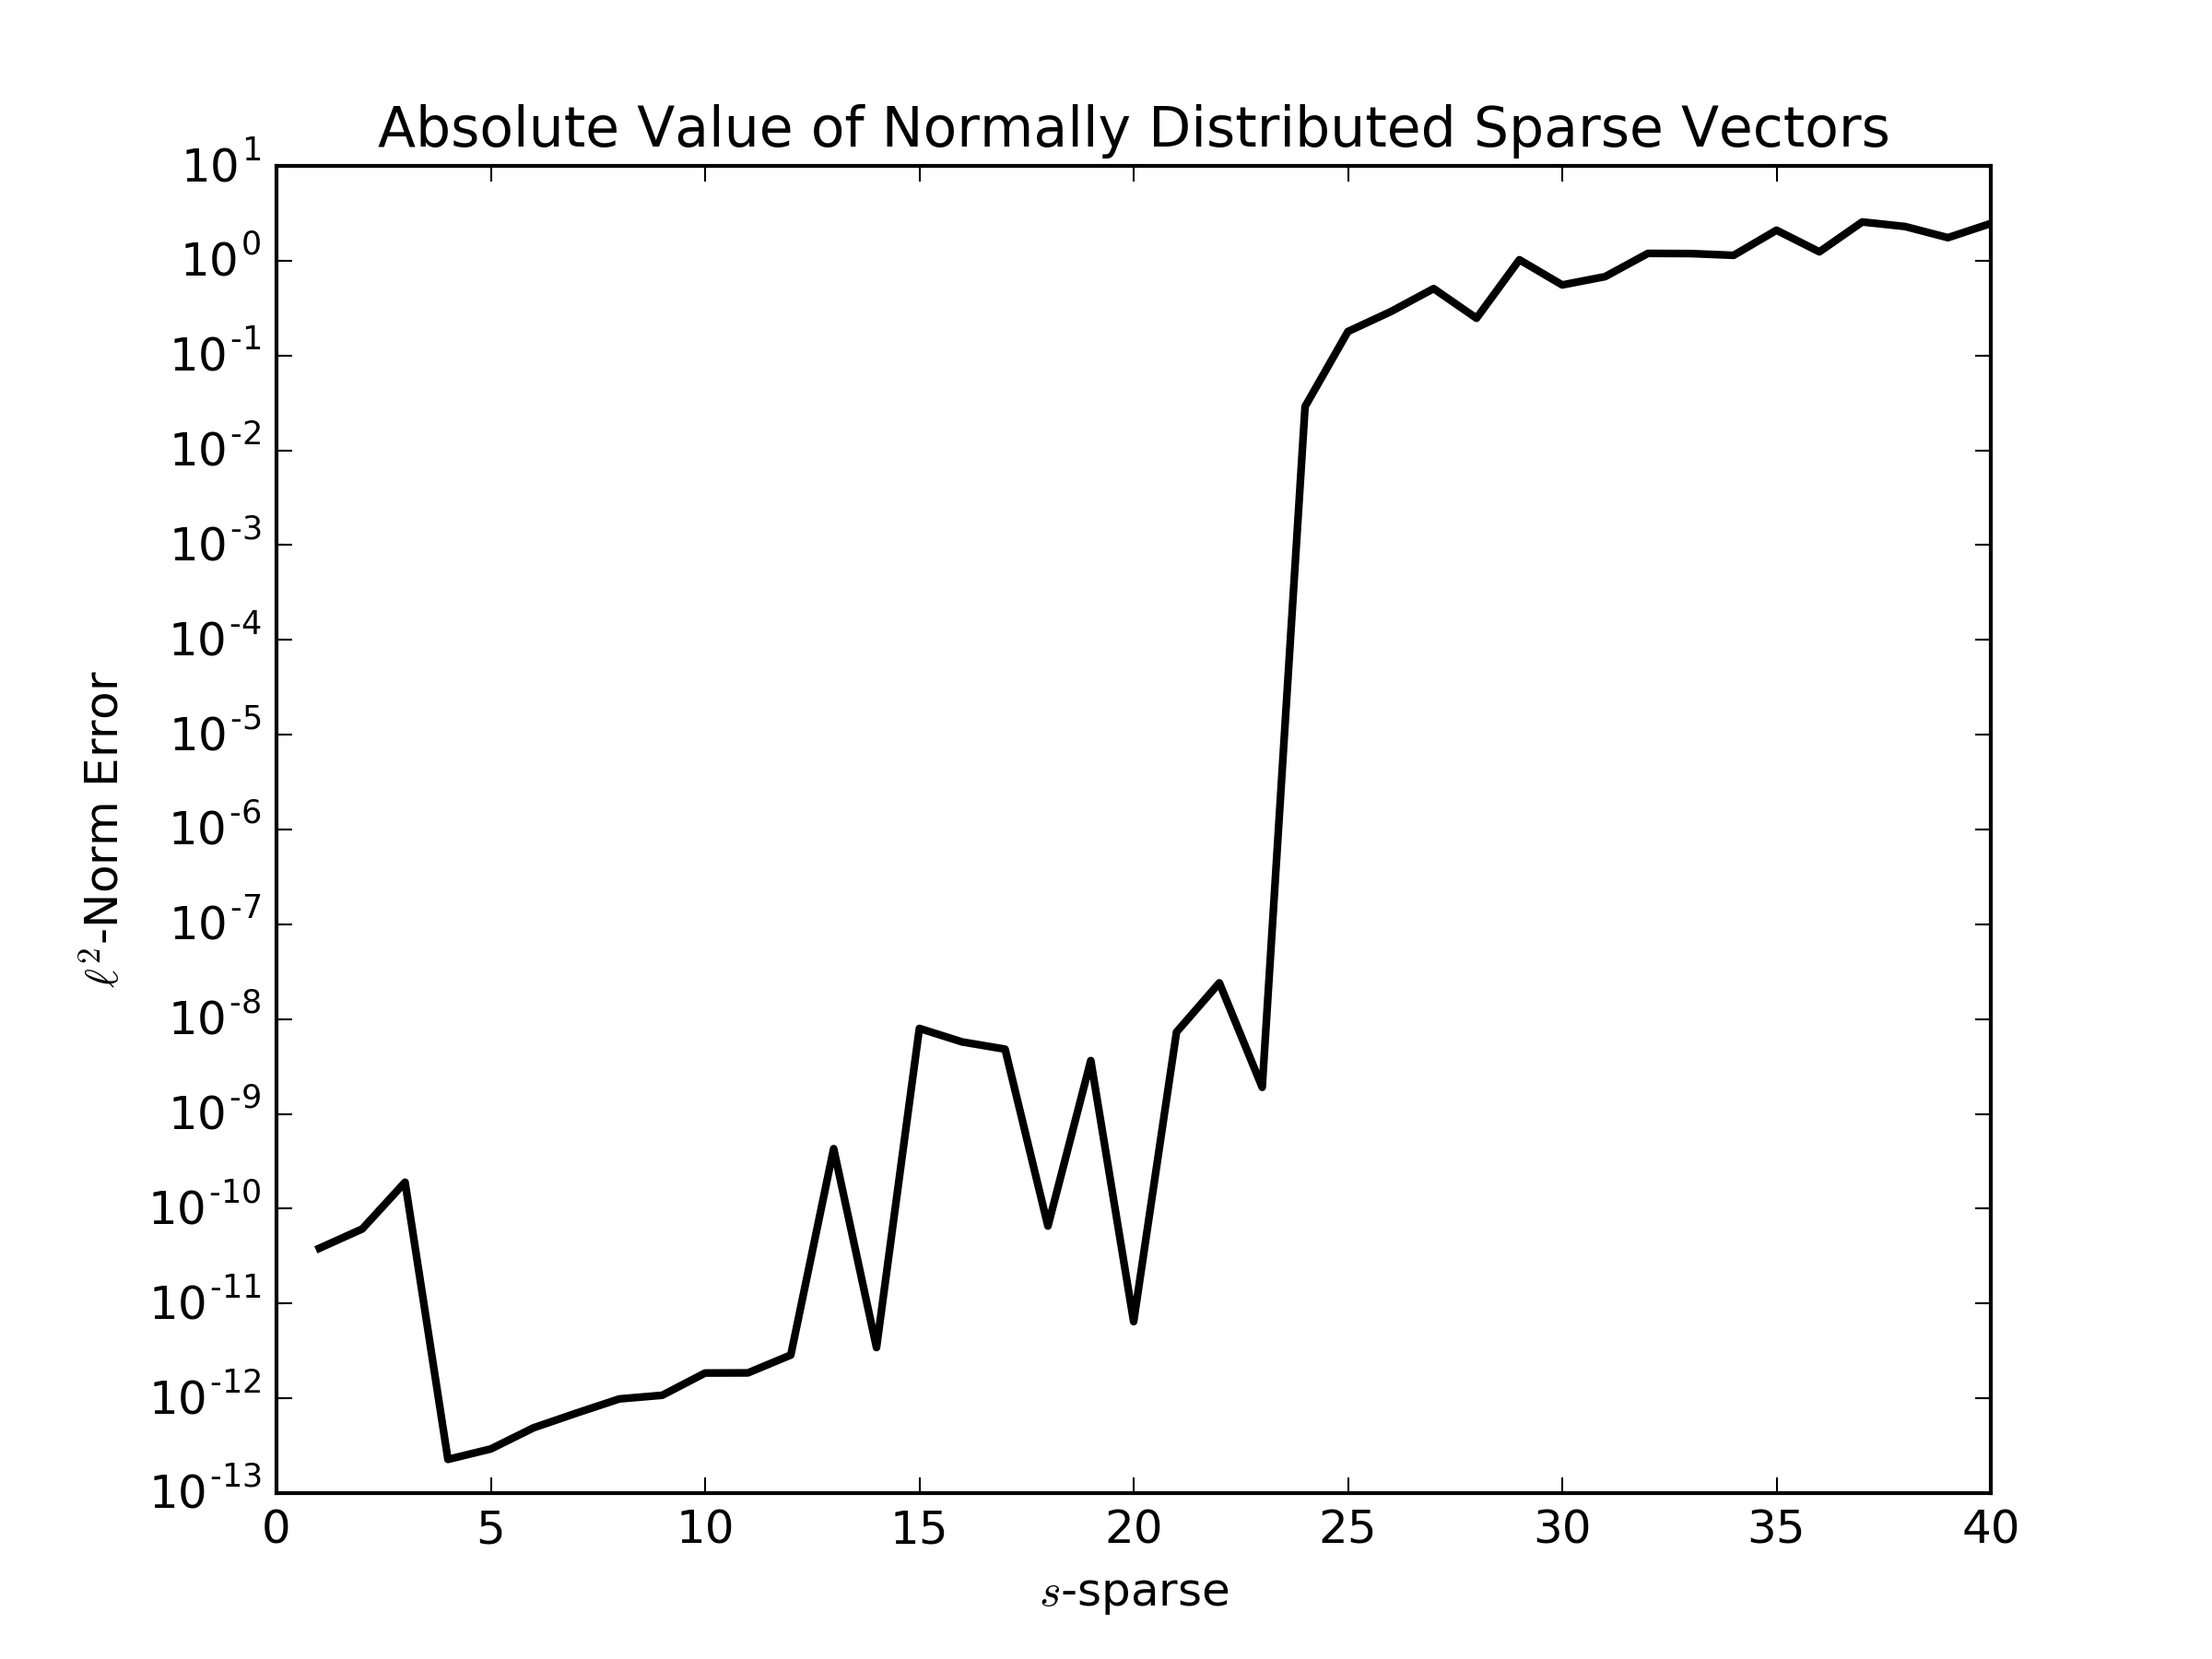
\includegraphics[width=\textwidth]{normally_distributed_nonnegative.png}
    \end{figure}
    In this experiment, this method failed for $s \geq 24$.
\end{proof}
    







\end{document}
